\documentclass[a4paper]{scrreprt}

\usepackage[german]{babel}
\usepackage[utf8]{inputenc}
\usepackage[T1]{fontenc}
\usepackage[titletoc]{appendix}
\usepackage{ae}
\usepackage{enumitem}
\usepackage[bookmarks,bookmarksnumbered]{hyperref}
\usepackage{graphicx}

\graphicspath{{resourcen/}}

%Used for including MetaUML diagrams
%\usepackage{emp}
%\usepackage{ifpdf}
%\ifpdf
\DeclareGraphicsRule{.1}{mps}{*}{}
%\fi

\makeatletter
\def\namedlabel#1#2{\begingroup
   #2%
   \def\@currentlabel{#2}%
   \label{#1}\endgroup
}

% Inhaltsverzeichnis Ebenen definieren, zB bis zu Subsection
\setcounter{secnumdepth}{4}
\setcounter{tocdepth}{1}

\usepackage[toc,acronym]{glossaries}
\makeglossaries

\usepackage{xparse}
\DeclareDocumentCommand{\newdualentry}{ O{} O{} m m m m } {
  \newglossaryentry{gls-#3}{name={#5},text={#5\glsadd{#3}},
    description={#6},#1
  }
  \makeglossaries
  \newacronym[see={[Glossary:]{gls-#3}},#2]{#3}{#4}{#5\glsadd{gls-#3}}
}

\newcounter{psnr}
\newcounter{nfanr}
\newcounter{fanr}
\newcounter{tnr}

\makeatother
\loadglsentries{glossary.tex}
\begin{document}

\title{Pflichtenheft\\
Graph von Ansicht}
\date{}
\author{Nicolas Boltz   \\ uweaw@student.kit.edu
  \and Jonas Fehrenbach \\ urdtk@student.kit.edu
  \and Sven Kummetz     \\ kummetz.sven@gmail.com
  \and Jonas Meier      \\ Meierjonas96@web.de
  \and Lucas Steinmann  \\ ucemp@student.kit.edu
}

\titlehead{\includegraphics[width=150pt]{resourcen/GAns.png}}

\maketitle

% Ich denke einen Abstract brauchen wir nicht aber hier ist mal ein Template einfach die Kommentarzeichen wegmachen
%\begin{abstract}
%\end{abstract}

\tableofcontents

\chapter{Zielbestimmung}

Graph von Ansicht soll Programmgraphen von externen Analyse-Programmen visualisieren. Dafür wird eine bereits vorhandene Graphdatei importiert und ausgewertet. Der Benutzer kann verschiedene Constraints einstellen, welche im weiteren Dokument näher erläutert werden. 
%TODO: Verweis einfügen zu den konkreten Erläuterungen
Das Endergebnis soll eine übersichtliche Darstellung der Abhängigkeiten und des Steuerflusses eines Programmes zeigen, das dem Benutzer die Möglichkeit bietet, das Programm besser analysieren zu können.

\section{Pflichtkriterien}

\begin{itemize}
\item Schnittstellen
\begin{itemize}
\item Import von generischen Graphen im \gls{graphml}-Format
\item Export der visualisierten Graphen im \gls{svg}-Format
\end{itemize}
\item User interface
\begin{itemize}
\item Navigation mittels Zoom und Translation
\item Selektieren von einzelnen oder mehreren Knoten
\item Einstellen von Constraints
\item Kollabieren und Ausklappen von Gruppen und Teilgraphen
\item Filter für Knoten- und Kantentypen
\item Ausblendung selektierter Knoten
\end{itemize}
\item Visualisierung
\begin{itemize}
\item Hierarchisches Layout mit dem \gls{sugiyama}
\item Kanten werden durch \gls{bezier} dargestellt
\item Informationsanzeige von Knoten und Kanten
\item Weitere Layoutalgorithmen sollen leicht integrierbar und austauschbar sein
\end{itemize}
\item Layout
\begin{itemize}
	\item Sprungpunkte (aka "Knubbel", wie bei yComp) etc...
	%evtl. genauer, anders, besser, mehr ... ;)
\end{itemize}
\end{itemize}

\section{Wunschkriterien}

\begin{itemize}
\item Schnittstellen
\begin{itemize}
\item Export der visualisierten Graphen im \gls{jpg}- und \gls{graphml}-Format
\item Erweiterbarkeit des Programmes durch Plugin Schnittstellen
\end{itemize}
\item User interface
\begin{itemize}
\item Muster Definition mittels "GraphRegex"
\item Benutzerdefinierte Hotkeys
\end{itemize}
\item Visualisierung
\begin{itemize}
\item Fortschrittsbalken bei Berechnung der Visualisierung des Graphen mithilfe einer Zeitabschätzung
\item Minimap bzw. Übersicht des Graphens
\item Algorithmus zur Erreichbarkeit eines Knoten
\item Die visuelle Darstellung von Kanten kann geändert werden (\gls{bezier}, orthogonale Kanten oder direkte Kanten)
\end{itemize}
\end{itemize}

\section{Abgrenzungskriterien}

\begin{itemize}
\item Das Produkt ist kein Graph Editor und unterstützt nicht das manuelle Zeichnen/Hinzufügen von neuen Kanten und Knoten.
\item Die GUI wird nicht von Grund auf neu entwickelt, es werden Bibliotheken verwendet, um die Entwicklung zu erleichtern. 
\item Das Darstellen von Kanten und Knoten selbst wird mithilfe von Bibliotheken umgesetzt.
\item Das Produkt ist kein Analysetool für Programme, sondern dient lediglich zur Visualisierung von bereits vorhandenen Graphdateien.
\end{itemize}

\chapter{Produkteinsatz}

\section{Anwendungsbereiche}
Graph von Ansicht soll zur Visualisierung von Programmgraphen eingesetzt werden. Der Nutzer soll dadurch die Abhängigkeiten und den Steuerfluss eines Programms besser verstehen.
\section{Zielgruppen}
Institute und Forschungsgruppen, die sich mit der Analyse von Programmen beschäftigen. Das Programm richtet sich auch an Menschen welche vorhandene Graphdateien visualisieren und sich mit dem Thema Programmgraphen vertraut machen wollen.

\section{Betriebsbedingungen}
Das Produkt besteht aus einem Graphviewer (Graph von Ansicht) und wird mit einem JOANA-Plugin ausgeliefert. Somit benötigt es keine weiteren Installationen (abgesehen von der \gls{jre}), damit es funktioniert. Es benötigt auch keine aktive Internetverbindung oder ein Netzwerk. Es wird lediglich eine Graphdatei als Input benötigt. Das Programm ist für Linux und Windows Betriebssysteme ausgelegt und funktioniert nur auf diesen garantiert (siehe \nameref{ch:umgebung}).

\chapter{Produktumgebung}
\label{ch:umgebung}

\section{Software}\label{sec:software}
Das Produkt muss in folgenden Desktop-Systemen ausführbar und, wie im restlichen Dokument beschrieben, benutzbar sein:
\begin{itemize}
  \setlength\itemsep{0em}
  \item Linux Fedora 22/23 %TODO nochmal die Versionen in der ATIS nachsehen und abgleichen.
  \item Linux Ubuntu 15.10/16.04 LTS
  \item Windows 7 und höher
\end{itemize}
Zur Programmierung wird die Programmiersprache Java benutzt. Daher ist eine Installation der \gls{jre} 8+ zur Ausführung notwendig.

\section{Hardware}
Das Produkt ist als \gls{jfx}-Anwendung zur Ausführung auf Desktop-Systemen konzipiert.
Durch die Verwendung von Java ist das Produkt unabhängig von Details der unterliegenden Hardware, sofern diese in der Lage ist, die benötigte \gls{jre} (siehe \ref{sec:software}) auszuführen.
Um die in Kapitel~\ref{ch:nfa} beschriebenen nichtfunktionalen Anforderungen einhalten zu können, sind folgende Mindestanforderungen an das System, auf dem das Produkt ausgeführt werden soll, notwendig:

\begin{itemize}
  \setlength\itemsep{0em}
  \item Arbeitsspeicher: 4 GB
  \item Prozessor: Intel Core i5-4210U %TODO Jonas F. Prozessor; vlt. durch gleichwertigen Desktopprozessor ersetzen.
  \item Festplattenspeicher: 200 MB 
  \item Display: 1280x960
\end{itemize}


\chapter{Plugin-Schnittstellen}
\label{ch:plugschnitt}

\setcounter{psnr}{10}
\newcommand{\psno}{\ifnum\value{psnr}<10 00\else\ifnum\value{psnr}<100 0\fi\fi\arabic{psnr}\addtocounter{psnr}{10}}
\renewcommand\thesubsubsection{/S\ifnum\value{psnr}<10 000\else\ifnum\value{psnr}<100 00\else\ifnum\value{psnr}<1000 0\fi\fi\fi\arabic{psnr}/}
\newcommand\ps[2]{\namedlabel{s:#1}{\textbf{/S\psno/}}: & #2 \\ [1ex] }

\begin{tabular}{lp{0.9\linewidth}}
  \ps{graphtyp}{\textit{Graphtypen-Schnittstelle:} Plugins sind in der Lage neue Graphtypen zu definieren. Alle von Plugins definierten Graphtypen sind dem Benutzer beim Importieren zur Auswahl gestellt. Das Plugin kann dann mit einem Graphtyp bestimmte Import-Möglichkeiten, Layoutalgorithmen, Darstellungsoptionen verbinden.
So dass der Benutzer diese nicht bei jedem Öffnen eines Graphen neu festlegen muss und gleichzeitig eine Importfunktion für ein Datenformat von mehreren Plugins wiedervewendet werden können.}
  \ps{import}{\textit{Import-Schnittstelle:} Ein Plugin welches auf diese Schnittstelle zugreift, kann ein neuen Datentyp festlegen, für welches es einen Importfunktion implementiert. Dieser steht dann in der Importfunktion von Graph von Ansicht zur Verfügung. Das Plugin soll in der Lage sein den neuen Datentyp zu parsen und an Graph von Ansicht weiterzuleiten.}
  \ps{export}{\textit{Export-Schnittstelle:} Graph von Ansicht sendet interne Daten über den gezeichneten Graphen an diese Schnittstelle. Das Plugin welches auf diese Schnittstelle zugreift soll in der Lage sein aus diesen Daten einen neuen Datentyp zu erstellen und abzuspeichern. Der Datentyp erscheint dann auch beim Speicherdialog}
  \ps{layoutalgo}{\textit{Layoutalgorithmen-Schnittstelle:} Bei dieser Schnittstelle kann ein neuer Algorithmus implementiert werden, auf welchen dann beim Layouten eines Graphens zugegriffen werden kann. Das Plugin bekommt eine interne Repräsentation des Graphens und soll jedem Knoten eine Koordinate zuordnen. Außerdem sollen die Züge von Kanten festgelegt werden.}
  \ps{filter}{\textit{Filter-Schnittstelle:} Es können neue Filter für spezielle Knoten- und Kantentypen hinzugefügt werden, welche bei den Filteroptionen von Graph von Ansicht automatisch hinzugefügt werden. Diese Filter bestehen darin, dass sie Kanten oder Knoten nach bestimmten Eigenschaften ausblenden.}
  \ps{darstellung}{\textit{Darstellungs-Schnittstelle:} Es können einzelnen Knoten- und Kantentypen Eigenschaften zugeordnet werden, wie zum Beispiel die Farbe für das Layout oder die Form oder zusätzliche Informationen, welche in der Informationsanzeige angezeigt werden.}
  \ps{operationen}{\textit{Operation-Schnittstelle für Knoten und Kanten:} Es können neue Operationen auf Knoten und Kanten ausgeführt werden, wie das Kollabieren von bereits definierten Teilgraphen (z.B. Feldzugriffe bei JOANA).}
\end{tabular}


\chapter{Funktionale Anforderungen}
\label{ch:funktionen}


\setcounter{fanr}{10}
\newcommand{\fano}[1]{\subsubsection{#1}\addtocounter{fanr}{10}}
\newcommand{\subfano}[1]{\subsubsection{#1}\addtocounter{fanr}{1}}
\renewcommand\thesubsubsection{/FA\ifnum\value{fanr}<10 00\else\ifnum\value{fanr}<100 0\fi\fi\arabic{fanr}/}

\section{Graph von Ansicht}

\subsection{Allgemein}

\fano{Anzeige von Graphen}\label{fa:graphen}
\textbf{Ziel:} Ein Graph soll in der Graphansicht angezeigt werden.\\
\textbf{Vorbedingung:} -\\
\textbf{Nachbedingung (Erfolg):} Der Graph ist in der Graphansicht sichtbar.\\
\textbf{Nachbedingung (Fehlschlag):} -\\
\textbf{Auslösende Ereignisse:}
\begin{enumerate}[nolistsep, label=(\alph*)]
  \item Eine Graphdatei wird importiert.
  \item Ein Graph wird aus der Struckturansicht ausgewählt.
\end{enumerate}
\textbf{Beschreibung:}\\
Importieren (a): Der in der Graphdatei zuerst beschriebene Graph, wird in der Graphansicht angezeigt.\\
Auswahl (b): Der ausgewählte Graph in der Graphansicht angezeigt.


\fano{Anzeige von geschachtelten Graphen}\label{fa:hierarchgraph}
\textbf{Ziel:} Falls ein Graph einen geschachtelten Graphen enthält, soll dieser angezeigt werden.\\
\textbf{Vorbedingung:} Eine Graphdatei mit geschachtelten Graphen wurde importiert.\\
\textbf{Nachbedingung (Erfolg):} Der geschachtelte Graph wird in der Graphansicht angezeigt.\\
\textbf{Nachbedingung (Fehlschlag):} -\\
\textbf{Auslösende Ereignisse:}
\begin{enumerate}[nolistsep, label=(\alph*)]
  \item Der Benutzer wählt den geschachtelten Graphen aus der Struckturansicht aus.
  \item Ein Graph mit einem geschachtelten Graphen wird in der Graphansicht angezeigt.
    Der Benutzer wählt die Funktion über das Kontextmenü des Knotens, der den geschachtelten Graphen enthält, aus oder löst sie durch ein Tastenkürzel aus.
\end{enumerate}
\textbf{Beschreibung:}\\
Geschachtelte Graphen werden in der Graphansicht als Knoten dargestellt.
Wenn der Benutzer einer der Ereignisse auslöst wird der Graph in der Graphansicht angezeigt.
Ein geschachtelter Graph wird in der Struckturansicht als Kind des Graphen dargestellt, der in enthält. Für ein Beispiel siehe hier:\\ %TODO: Referenz von GUI Bild mit Struckturansicht
Ein geschachtelter Graph wird in der Graphansicht wie ein ``Top-Level-''Graph behandelt.


\fano{Graphen layouten}\label{fa:layout}
\textbf{Ziel:} Ein Graph soll nach bestimmten Vorgaben bzw. einem bestimmten Muster angeordnet werden.\\
\textbf{Vorbedingung:} Ein Graph wurde in die Graphansicht geladen.\\
\textbf{Nachbedingung (Erfolg):} Allen Knoten wurden bestimmte Positionen zugeordnet. Kanten wurden feste Züge zugewiesen.\\
\textbf{Nachbedingung (Fehlschlag):} -\\
\textbf{Auslösende Ereignisse:}
Der Benutzer wählt über die Menüleiste ein Layout aus.\\
\textbf{Beschreibung:}\\
Nach der Auswahl wird das Layout berechnet. Hierbei kann es zu Verzögerungen kommen. (siehe \ref{nfa:berechzeit})
Nach der Berechnung wird der Graph neugezeichnet. Layouts sind nicht in Graph von Ansicht enthalten und können durch Plugins hinzugefügt werden.
Dem Produkt werden über das JOANA-Plugin Layout zur Darstellung von, von \gls{joana} berechneten, SDGs mitgeliefert.
Diese Layouts muss alle Anforderungen beschrieben in \ref{sec:nfajoana} erfüllen.

\subsection{User Interface}
\setcounter{fanr}{100}

\fano{Sichtfeld verschieben}\label{fa:verschieben}
\textbf{Ziel:} Das Sichtfeld soll verschoben werden.\\
\textbf{Vorbedingung:} Ein Graph wurde in die Graphansicht geladen und das Sichtfeld deckt nicht alle Elemente des Graphens ab.\\
\textbf{Nachbedingung (Erfolg):}  Das Sichtfeld deckt nun den gewünschten Teil des Graphen ab.\\
\textbf{Nachbedingung (Fehlschlag):} Das Sichtfeld deckte einen Randabschnitt ab und es wurde versucht das Sichtfeld über den Rand hinaus zu bewegen.\\
Das Sichtfeld wird nicht über den Rand bewegt. Es wird keine Fehlermeldung ausgegeben.\\
\textbf{Auslösende Ereignisse:}
\begin{enumerate}[nolistsep, label=(\alph*)]
  \item Der Benutzer klickt und zieht mit der mittleren Maustaste in einem leeren Bereich des Graph-Fenster.
  \item Der Benutzer betätigt eine der zum Verschieben des Sichtfeldes designierten Tasten \ref{fa:hotkey}
  \item Der Benutzer bewegt die Scroll-Balken am Rand des Sichtfeldes. % TODO: Referenzt auf GUI Entwurf, wo scrollbalken sichtbar sind
\end{enumerate}
\textbf{Beschreibung:}\\
Klicken und Ziehen (a): Das Sichtfeld bewegt sich entgegen der Richtung, in welche der Mauszeiger bewegt wird. Es entsteht somit ein intuitives Verschieben des Graphen.\\
Navigationstasten (b): Das Sichtfeld verschiebt sich um eine feste Länge (in Abhängigkeit des Zoom-Grades) in die entsprechnde Richtung.\\
Scroll-Balken (c): Das Sichtfeld bewegt sich relativ zur Größe des gesamten Graphen um das gleiche Maß wie der Scroll-Balken zur Länge seiner Fahrbahn in die entsprechende Richtung (Horizontal/Vertikal).\\

\fano{Zoom-Grad ändern}\label{fa:zoom}
\textbf{Ziel:} Der Zoom-Grad des Sichtfeldes soll vergrößert bzw. verkleinert werden.\\
\textbf{Vorbedingung:} Ein Graph wurde geladen in die Graphansicht.\\
\textbf{Nachbedingung (Erfolg):} Der Zoom-Grad wurde angepasst.\\
\textbf{Nachbedingung (Fehlschlag):} Der Zoom-Grad bleibt gleich, falls ein Maximum/Minimum erreicht wurde. Es wird keine Fehlermeldung ausgegeben.\\
\textbf{Auslösende Ereignisse:}
\begin{enumerate}[nolistsep, label=(\alph*)]
  \item Der Benutzer dreht am Mausrad.
  \item Der Benutzer betätigt die zum Zoomen designierten Tasten. \ref{fa:hotkey}
\end{enumerate}
\textbf{Beschreibung:}\\
Mausrad (a): Der Zoom-Grad ändert sich mit dem Drehen des Mausrades. Die Änderungsrichtung kann sich in Abhängigkeit vom Betriebssystem ändern.\\
Zoom-Tasten (b): Der Zoom-Grad ändert sich um einen in Abhängigkeit zum derzeitigen Zoom-Grad festen Wert.\\

\fano{Knoten selektieren}\label{fa:selekt_knoten}
\textbf{Ziel:} Ein oder mehrere Knoten sollen der Auswahl hinzugefügt werden.\\
\textbf{Vorbedingung:} Ein Graph wurde in die Graphansicht geladen.\\
\textbf{Nachbedingung (Erfolg):} Ein oder mehrere Knoten wurden der Auswahl hinzugefügt.\\
\textbf{Nachbedingung (Fehlschlag):} -\\
\textbf{Auslösende Ereignisse:}
\begin{enumerate}[nolistsep, label=(\alph*)]
  \item Der Benutzer klickt mit der linken Maustaste auf einen Knoten.
  \item Der Benutzer klickt mit der linken Maustaste in einen leeren Bereich des Sichtfeldes und zieht den Mauszeiger.
\end{enumerate}
\textbf{Beschreibung:}\\
Der Benutzer kann Knoten mit der Maus zur Auswahl hinzufügen.
Auf eine Auswahl von Knoten können verschiedene Funktionen ausgeführt werden. %TODO: Referenz auf Funktionen auf Knotenmengen/Teilgraphen
Die derzeit ausgewählten Knoten werden graphisch hervorgehoben.\\

\fano{Knoten und Kanten filtern}\label{fa:filter}
\textbf{Ziel:} Knoten und Kanten können bezüglich ihres Types gefiltert werden.\\
\textbf{Vorbedingung:} Ein Graph wurde geladen.\\
\textbf{Nachbedingung (Erfolg):} Es wurden Knoten und Kanten eines bestimmten Types ein-/ausgeblendet.\\
\textbf{Nachbedingung (Fehlschlag):} -\\
\textbf{Auslösende Ereignisse:}
Der Benutzer wählt die Filter-Funktion aus dem Menüleiste aus.\\
\textbf{Beschreibung:}
Der Benutzer kann aus einer Reihe von Filtern auswählen.
Mitgeliefert werden über das JOANA-Plugin folgende Filter: % Referenz Plugin
\begin{itemize}[nolistsep]
  \item Kontrollfluss
  \item Kontrollabhängigkeit
  \item Datenabhängigkeit
  \item Heap-Abhängigkeiten
  \item Parameterstruktur
  \item Threadinterferenzen
\end{itemize}
Die Kanten werden entsprechend aus- oder eingeblendet.\\
\textbf{Alternative:}
Der Graph wird neugezeichnet um kompakter zu werden oder um Platz für neue Kanten zu machen.

\fano{Wechsel zwischen Graphen}\label{fa:graphwechsel}
\textbf{Ziel:} Der in der Graphansicht angezeigte Graph wurde ausgetauscht. \\
\textbf{Vorbedingung:} Eine Graphdatei wurde geladen.\\
\textbf{Nachbedingung (Erfolg):} Der ausgewählte Graph wird in der Graphansicht angzeigt.\\
\textbf{Nachbedingung (Fehlschlag):} -\\
\textbf{Auslösende Ereignisse:}
Der Benutzer wählt über die Graph-Übersicht einen anderen Graphen aus.\\
\textbf{Beschreibung:}
Das Produkt unterstützt Graphdateien, welche mehr als einen Graphen beschreiben.
Mit dieser Funktion kann der Benutzer die Ansicht zwischen den Graphen wechseln.

\fano{Steuerung über Tastaturkürzel}\label{fa:hotkey}
\textbf{Ziel:} Häufig verwendete Funktionen können über Tastaturkürzel ausgeführt werden.\\
\textbf{Vorbedingung:} -\\
\textbf{Nachbedingung (Erfolg):} Die dem Tastaturkürzel zugeordnete Funktion wurde ausgeführt.\\
\textbf{Nachbedingung (Fehlschlag):} -\\
\textbf{Auslösende Ereignisse:}
Ein Benutzer aktiviert ein Tastenkürzel, welchem eine Funktion zugeordnet ist.\\
\textbf{Beschreibung:}
Vom Benutzer ausführbare Funktionen (wie z.B. Navigation im Graphen) und Menüs sind Tastaturkürzel zugeordnet.
Die Tastenkürzel werden hinter dem Funktionsnamen im Menüleiste oder Kontextmenü angezeigt.

\section{\gls{graphml}-Plugin}

\fano{Graph aus Datei importieren}\label{fa:import}
\textbf{Ziel:} Der in der Graphdatei beschriebene Graph soll visuell dargestellt werden.\\
\textbf{Vorbedingung:} Der Benutzer hat eine unterstützte Graphdatei (siehe \ref{ch:daten}) in seinem Dateissystem, auf welche zugegriffen werden kann.\\
\textbf{Nachbedingung (Erfolg):} Der Graph wird dargestellt.\\
\textbf{Nachbedingung (Fehlschlag):}
Eine Fehlermeldung wird ausgegeben, dass die Datei nicht geöffnet werden konnte, bzw. dass die Datei keinen korrekten Graph beschreibt.\\
\textbf{Auslösende Ereignisse:}
\begin{enumerate}[nolistsep, label=(\alph*)]
  \item Der Benutzer wählt die Import-Funktion über das Menüband aus, nachdem das Programm geöffnet wurde. %TODO: Referenz zu Menüband in GUI
  \item Der Benutzer ruft das Programm auf und übergibt den Pfad zur Graphdatei als Argument. %TODO: Benutzerschnittstelle Kommandozeile
\end{enumerate}
\textbf{Beschreibung:}\\
Menüband (a): Ein Dateiverzeichnis-Menü öffnet sich. %TODO: Dateiverzeichnis-Menü auch in GUI-Entwurf oder klar?
Der Benutzer wählt die zu importierende Datei aus.
Der in der Datei beschriebene Graph wird im Graph-Fenster dargestellt.\\%TODO: % Referenz zur GUI (Graph-Fenster)
Kommandozeilenargument (b): Der Graph wird gleich nach dem Programmstart im Graph-Fenster dargestellt.

\section{\gls{svg}-Plugin}

\fano{Export als Bilddatei}\label{fa:export_img}
\textbf{Ziel:} Der Graph soll in seiner aktuellen Darstellung als Bilddatei exportiert werden.\\
\textbf{Vorbedingung:} Ein Graph wurde geladen. \\
\textbf{Nachbedingung (Erfolg):} Es wurde eine Bilddatei an einer gewünschten, schreibbaren Stelle im Dateissystem erstellt, welche ein Abbild des derzeit angezeigten Graphens enthält.\\
\textbf{Nachbedingung (Fehlschlag):} Die Bilddatei konnte nicht erstellt werden. Es wird eine Fehlermeldung ausgegeben.\\
\textbf{Auslösendes Ereignis:}
Der Benutzer wählt die Exportfunktion im Menübalken aus.\\
\textbf{Beschreibung:}\\
Der Benutzer wählt die Exportfunktion im Menübalken unter Datei-->Export--><Dateiformat> aus. Wobei <Dateiformat> durch das gewünschte Bilddatei-Format zu ersetzen ist. Unterstützt wird mindestens das \gls{svg}-Format. %TODO: Referenz auf Dateiformate und Erweiterbarkeit durch Plugins
Es erscheint ein Dateisystem-Menü indem, der Pfad zum Abspeichern der Bilddatei ausgewählt werden kann.
Eventuell wird der Benutzer nach weiteren, zur Abspeicherung relevanten, Details abgefagt. (z.B. Stärke der Komprimierung bei JPEG) %TODO: Durch Beispiel in SVG ersetzten
Es wird versucht die Bilddatei am ausgewählten Ort abzuspeichern.\\

\section{\gls{joana}-Plugin}



%\fano{<++>}\label{fa:<++>}
%\textbf{Ziel:} <++>\\
%\textbf{Kategorie:} <++>\\
%\textbf{Vorbedingung:} <++>\\
%\textbf{Nachbedingung (Erfolg):} <++>\\
%\textbf{Nachbedingung (Fehlschlag):} <++>\\
%\textbf{Auslösende Ereignisse:}
%\begin{enumerate}[nolistsep, label=(\alph*)]
%  \item <++>
%\end{enumerate}
%\textbf{Beschreibung:}
%\begin{enumerate}[nolistsep]
%  \item <++>
%\end{enumerate}
%\textbf{Alternativen:}
%\begin{enumerate}[nolistsep]
%  \item <++>
%\end{enumerate}


\chapter{Produktdaten}\label{ch:daten}

\begin{itemize}
  \item Seit Programmstart gesetzte Einstellungen (z.B. Speicherort der zuletzt exportierten Datei oder Größe des Fensters) werden mithilfe der \gls{prefapi} von Java gespeichert.
  \item Als Inputformat für die zu zeichnenden Graphen wird das \gls{graphml}-Format unterstützt.\\
    Das GraphML-Format ist so aufgebaut, dass nicht alle Konstrukte welche mit GraphML beschrieben werden können (wie z.B. \gls{hyperkante}),
    von einer Applikation unterstützt werden müssen.
    Nicht unterstützte Konstrukte können ignoriert werden, ohne strukturelle Informationen des restlichen Graphens zu verlieren.\\
    Wir listen hier die GraphML-Konstrukte, welche von dem Produkt unterstützt werden müssen und für welche eventuell eine Unterstützung später hinzugefügt wird, auf:
    \begin{itemize}
      \item Muss-Konstrukte: graph, node, edge, desc, key, data, default, Hierarchische/Geschachtelte Graphen  % Ist Port ein Musskriterium? Beim ersten Treffen wurde es erwähnt
      \item Kann-Konstrukte: hyperedge, port, endpoint, Multi-Graphen
    \end{itemize}
    Für den Fall das ein Kann-Konstrukt nicht unterstützt wird, wird es, wie in der GraphML Spezifikation vorgeschrieben, behandelt.
  \item Das Produkt wird den resultierenden Graphen als \gls{svg}-Format exportieren können.
\end{itemize}


\chapter{Nichtfunktionale Anforderungen}
\label{ch:nfa}

\newcounter{nfanr}[chapter]
\setcounter{nfanr}{10}
\newcommand{\nfano}{\ifnum\value{nfanr}<10 00\else\ifnum\value{nfanr}<100 0\fi\fi\arabic{nfanr}\addtocounter{nfanr}{10}}
\renewcommand\thesubsubsection{/NFA\ifnum\value{nfanr}<10 000\else\ifnum\value{nfanr}<100 00\else\ifnum\value{nfanr}<1000 0\fi\fi\fi\arabic{nfanr}/}
\newcommand\nfa[2]{\namedlabel{nfa:#1}{\textbf{/NFA\nfano/}}: & #2 \\}

\begin{tabular}{lp{0.9\linewidth}}
  \nfa{maxknoten}{Zu jedem Zeitpunkt können nicht mehr als 10.000 Knoten gleichzeitig gelayoutet und dargestellt werden. Dies entspricht nicht der maximalen Knotenzahl von SDGs die unterstützt werden.}
  \nfa{maxknotentotal}{Es werden Graphen mit nicht mehr als 1.000.000 Knoten insgesamt unterstützt.}
\end{tabular}


\chapter{Benutzerschnittstellen}

\section{Kommandozeile}

Die Kommandozeilen-Schnittstelle bietet dem Benutzer eine schnelle Möglichkeit Graphdateien beim Programmstart mit zusätzlichen Parametern zu öffnen.
Folgende Parameter werden unterstützt:\\
\subsection{Muss-Argumente}
\begin{tabular}{lp{0.75\linewidth}}
  -layout <layout> & Legt einen Layout-Algorithmus fest, welcher beim Programmstart auf den ersten Graphen angewendet wird.\\
    & Dabei ist <layout> ein Kürzel, das vom jeweiligen Layout-Plugin definiert wird. Das Kürzel wird hinter der Layout-Option in der Menüleiste angezeigt.\\
  -in <datei> & Legt die zu öffnende Graphdatei fest. <datei> ist der relative oder absolute Pfad zu einer Graphdatei. Alternativ kann ``-in'' weggelassen werden, falls der Pfad als letztes Argument angegeben wird.\\
\end{tabular}

\subsection{Kann-Argumente}
\begin{tabular}{lp{0.75\linewidth}}
  -out <datei> & Legt einen Pfad zu einer Datei fest, in welcher der Graph gespeichert werden soll.
  Es wird die in %TODO: Referenz zu Kann Funktion zum speichern von graphen
  beschrieben Funktion ausgeführt.
  Falls angegeben, wird der Layout-Algorithmus auf alle Graphen in der zu öffnenden Datei angewendet, bevor das Speichern beginnt.
  Die \gls{gui} wird nicht gestartet.
\end{tabular}

\section{GUI}


\chapter{Globale Testfälle}\label{ch:test}

\newcounter{stnr}
\setcounter{tnr}{10}

\newcommand{\testno}{\ifnum\value{tnr}<10 00\else\ifnum\value{tnr}<100 0\fi\fi\arabic{tnr}}
\newcommand\test[2]{\namedlabel{test:#1}{\textbf{/T\testno/}}\addtocounter{tnr}{10}\setcounter{stnr}{1} \hspace*{0.003\linewidth} \textbf{#2} \\ \\}

\newcommand\subtest[3]{\textbf{\arabic{stnr}}\addtocounter{stnr}{1}. & \textbf{Stand:} & #1 \\ & \textbf{Aktion:} & #2 \\ & \textbf{Reaktion:} & #3 \\ [1ex] }

\test{importJOANA}{Import und Darstellung von einem JOANA Graphen} 
\begin{tabular}{llp{0.9\linewidth}}
	\subtest
		{Graph von Ansicht ist gestartet und es wird kein Graph dargestellt}
		{Den Menüeintrag Datei->Import auswählen}
		{Ein Dateiauswahldialog wird geöffnet.}
	\subtest
		{Eine von JOANA exportierte Datei wurde im Dateisystem ausgewählt}
		{Button zum Laden der ausgewählten Datei drücken}
		{Der Dateiauswahldialog schließt sich und ein Dialog zur Auswahl des Layoutalgorithmus öffnet sich.}
	\subtest
		{Der Dialog zur Auswahl des Layoutalgorithmus wird angezeigt}
		{Der JOANA-Algorithmus wird ausgewählt und Ok gedrückt}
		{Der Dialog schließt sich und der \gls{callgraph} der geladen Datei wird im passenden Layout (siehe \ref{fa:layout}) angezeigt.}
\end{tabular}
\\ \\ \\
\test{openmethod}{Öffnen eines JOANA-Methodengraphen}
\begin{tabular}{llp{0.9\linewidth}}
	\subtest
		{Ein JOANA-Graph wurde importiert, der \gls{callgraph} wird angezeigt (siehe Test \ref{test:importJOANA}).}
		{Doppelklick auf einen Callknoten in der Strukturansicht.}
		{Ein neuer Tab öffnet sich, in dem der \gls{methgraph} auf den der Knoten verweist in passendem Layout dargestellt wird.}
	\subtest
		{Ein \gls{methgraph} wird dargestellt.}
		{In der Tableiste über der Graphansicht den ursprünglichen \glspl{callgraph} aus Schritt 1. auswählen.}
		{Der \gls{callgraph} des JOANA-Imports aus Schritt 1. wird wieder angezeigt.}
	\subtest
		{Der \gls{callgraph} wird angezeigt.}
		{Rechte Maustaste auf einen Callknoten.}
		{Das Kontextmenü für den selektierten Knoten öffnet sich.}
	\subtest
		{Das Kontextmenü für den Knoten wird angezeigt.}
		{Den Menüeintrag Öffnen auswählen.}
		{Ein neuer Tab öffnet sich, oder bei selber Auswahl wie in Schritt 1. wird zu dem bereits offenen Tab gewechselt, in dem der \gls{methgraph} auf den der Knoten verweist in passendem Layout dargestellt wird.}
\end{tabular}
\\ \\ \\
\test{navigation}{Navigation und Zoom}
\begin{tabular}{llp{0.9\linewidth}}
	\subtest
		{Ein JOANA-Graph wurde importiert und einer der enthaltenen \glspl{methgraph} oder \glspl{callgraph} wird angezeigt (siehe Test \ref{test:importJOANA}, \ref{test:openmethod}).}
		{Den Menüeintrag Ansicht->Zoom->Erhöhen auswählen.}
		{Der Mauszeiger ändert sich zu einer Lupe mit einem Plus in der Linse.}
	\subtest
		{Der Mauszeiger zeigt eine Lupe und befindet sich über der Graphansicht.}
		{Linksklick innerhalb der Graphansicht, in die nähe eines \glspl{subgraph}}
		{Das vorherige Sichtifeld wurde, in Richtung der Knoten und Kanten die in der Nähe des Mauszeigers beim Klick waren, herangezoomt.}
	\subtest
		{Der angezeigte Graph wird leicht herangezoomt dargestellt.}
		{Mittlere Maustaste in einem leeren Bereich der Graphansicht drücken und halten und ziehen des Mauszeigers.}
		{Das Sichtfeld wird, wenn nicht der Rand des Graphen erreicht wurde entgegen der Richtung in die der Mauszeiger bewegt wird, verschoben.}
%	\subtest{herauszoomen}
%	\subtest{kollabieren}
%	\subtest{ausklappen}
\end{tabular}
\\ \\ \\
\test{select}{Selektieren mehrerer Knoten und Kanten}
\begin{tabular}{llp{0.9\linewidth}}
	\subtest
	{Ein JOANA-Graph wurde importiert und einer der enthaltenen \glspl{methgraph} oder \glspl{callgraph} wird angezeigt.}
	{Selektieren eines \glspl{subgraph}, durch ziehen oder einzelnem Auswählen.}
	{Die ausgewählten Knoten und Kanten sind selektiert und visuell leicht hervorgehoben. Unter der Strukturansicht werden Informationen und Statistiken zu den selektierten Knoten und Kanten angezeigt.}
\end{tabular}
\\ \\ \\
\test{constraint}{Constraint zu Knoten eines geladenen Graphen hinzufügen}
\begin{tabular}{llp{0.9\linewidth}}
	\subtest
		{Ein JOANA-Graph wurde importiert und einer der enthaltenen \glspl{methgraph} oder \glspl{callgraph} wird angezeigt (siehe Test \ref{test:importJOANA}, \ref{test:openmethod}). Mindestens zwei Knoten auf unterschiedlichen Ebenen wurden selektiert (siehe Test \ref{test:select})}
		{Rechte Maustaste auf einen der selektierten Knoten.}
		{Das Kontextmenü für die selektierten Knoten öffnet sich.}
	\subtest
		{Kontextmenü wird angezeigt.}
		{Den Menüeintrag Constraint hinzufügen auswählen.}
		{Ein Dialog öffnet sich.}
	\subtest
		{Der Dialog zum Hinzufügen neuer Constraints ist geöffnet.}
		{Auswählen des Constraints zum nebeneinander Darstellen der Knoten und bestätigen des Dialogs.}
		{Der Dialog schließt sich. Der Graph wird neu gelayoutet und die zuvor selektierten Knoten werden nebeneinander in der gleichen Zeile dargestellt.}
\end{tabular}
\\ \\ \\
\test{exportSVG}{Export von einem geladenen JOANA-Graphen als SVG}
\begin{tabular}{llp{0.9\linewidth}}
	\subtest
		{Ein JOANA-Graph wurde importiert und einer der enthaltenen \glspl{methgraph} oder \glspl{callgraph} wird angezeigt (siehe Test \ref{test:importJOANA}, \ref{test:openmethod}).}
		{Den Menüeintrag Datei->Export->\gls{svg} auswählen.}
		{Es öffnet sich ein Dateiauswahldialog.}
	\subtest
		{Speicherort und Name der zu exportierenden Datei wurde im Dialog angegeben.}
		{Button zum Exportieren drücken.}
		{Der Dateiauswahldialog wird geschlossen, eine \gls{svg}-Datei mit dem angegebenen Namen wurde am ausgewählten Ort erstellt und sie enthält die visuelle Repräsentation des gesamten Graphen wie in der Graphansicht dargestellt wurde.}
\end{tabular}


\chapter{Systemmodelle}
\label{ch:sysmodel}

\section{Anwendungsfälle}
\begin{figure}[ht]
	\centering
	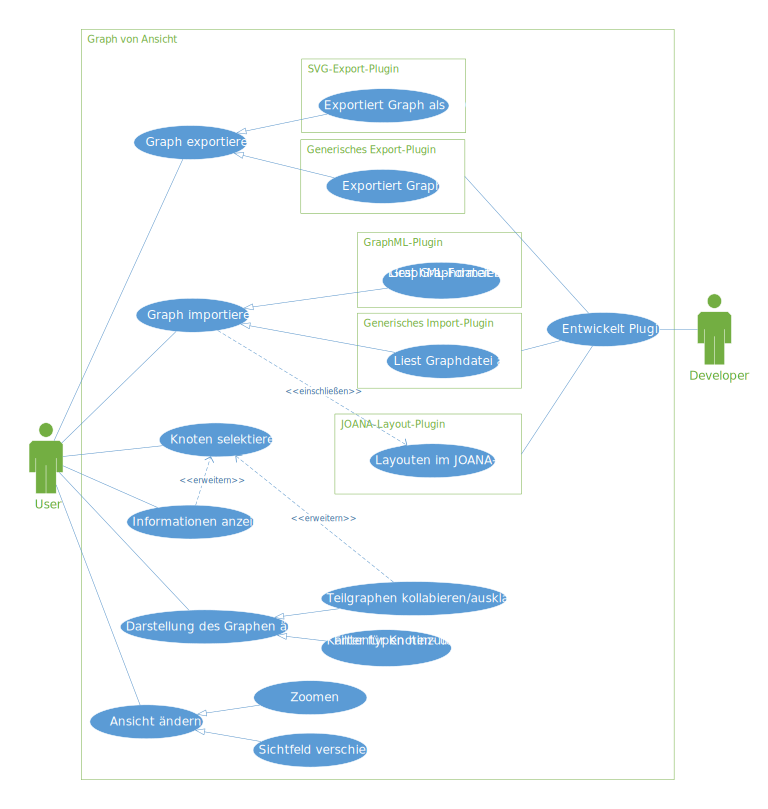
\includegraphics[width=310pt]{resourcen/usecase.png}
	\caption{Anwendungsfalldiagramm}
	\label{fig:usecase}
\end{figure}

\clearpage
\printglossary[type=\acronymtype]
\printglossary[title=Glossar,toctitle=Glossar]

\listoffigures

\end{document}
